\section{Experiment}
%if we do any practical experiments, what did we learn.
%Its important to keep the key elements of digital forensics in mind:
%\begin{itemize}
%\item evidence integrity
%Evidence integrity refers to the preservation of the evidence in its original form. This is a requirement that is valid both for the original evidence and the image.
%\item Chain of custody
%Chain of custody refers to the documentation of evidence acquisition, control, analysis and disposition of physical and electronic evidence.
%\item Forensically sound
%The term forensically sound methods and tools usually refers to the fact that the methods and tools adhere to best practice and legal requirements
%\end{itemize}
%automating is a possibility, some sort of "sorting" by cookie or 
%altering binary files in transmission to include a simple "call home with interesting information" addition.
%outgoing smtp = cleartext
%tcpdump -vv -x -X -s 1500 -i eth1 'port 25'
%port 25/smtp, verbose, print data of each packet, 
%http = cleartext.
We decided to set up a TOR exit node using Puppet for easy configuration, and reduced the ports it should allow to the ones we were most interested in. We decided that we were mostly interested in content on the following ports:\\

\begin{itemize}
	\item 22 - SSH traffic
	\item 23 - TELNET traffic
	\item 25 and 26 - SMTP traffic
	\item 80 - Default web port
	\item 443 - SSL traffic which could perhaps be useful for MITM attacks
	\item 6667 - Default IRC port
	\item 6697 - Default SSL IRC port
	\item 8888 and 8080 - Common ports for custom web interfaces
\end{itemize}

After setting up the exit node configuration, we set TCPdump to listen and dump traffic into a plethora of different \textit{.pcap} files. These files we could then use for inspecting packets and follow TCP streams in Wireshark.\\

\subsection{Analyzing captured data}
To further analyze interesting traffics in these files, we could run \textit{p0f}, the passive OS fingerprinting tool to retrieve some further information on a target, mainly the operating system used by the source. Something that makes it rather difficult to do this with TOR traffic is that we can't sort targets based on source IP addresses. This is a result of how TOR creates a path in the onion router network.\\

A useful tool for managing large amounts of captured network traffic for analysis is Xplico, which we attempted to run on our 19Gb of captured data. This turned out a failure unfortunately - although all data was supposedly decoded, the DeMa process (DecodingManager) suffered segmentation-faults, dumped its core, and thus it could not proceed to properly sort it out for analysis. Since the data was stored in a pcap file, it is possible to open it with Wireshark, but because of the size of it, this became much more complicated with the resources available on our machine, and left us lost in an abyss of information.\\

Still, as an example of how sniffed traffic can be used to identify some information on random targets which can then be filtered out to (hopefully) find what one is looking for, we have this:\\

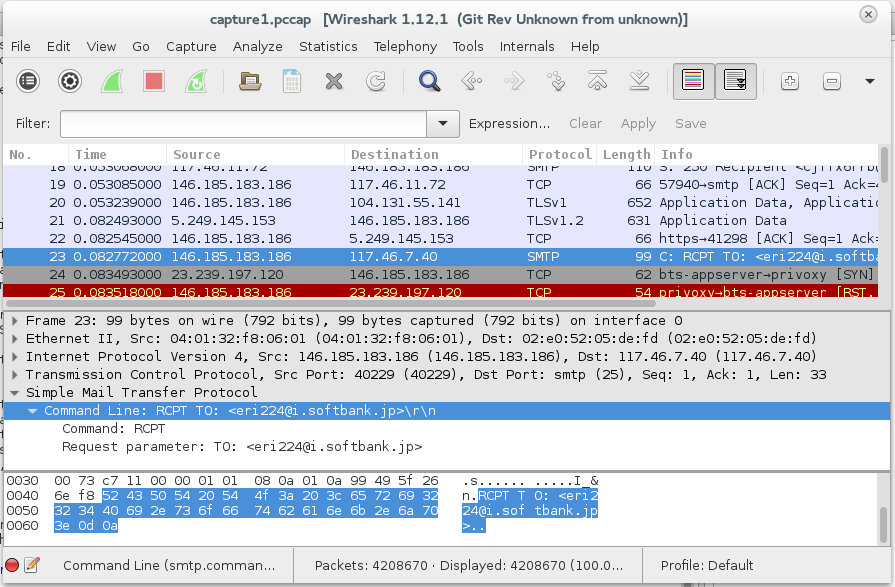
\includegraphics[scale=0.5]{wireshark.png}

Although this is messy, scavenging this for usernames is simple, and if any identifiers such as cookies, session IDs, etc are found together with these usernames, they could be used to dig up more information. Again, finding specific targets this way is sub-optimal, and reverse connections would be preferable.\\

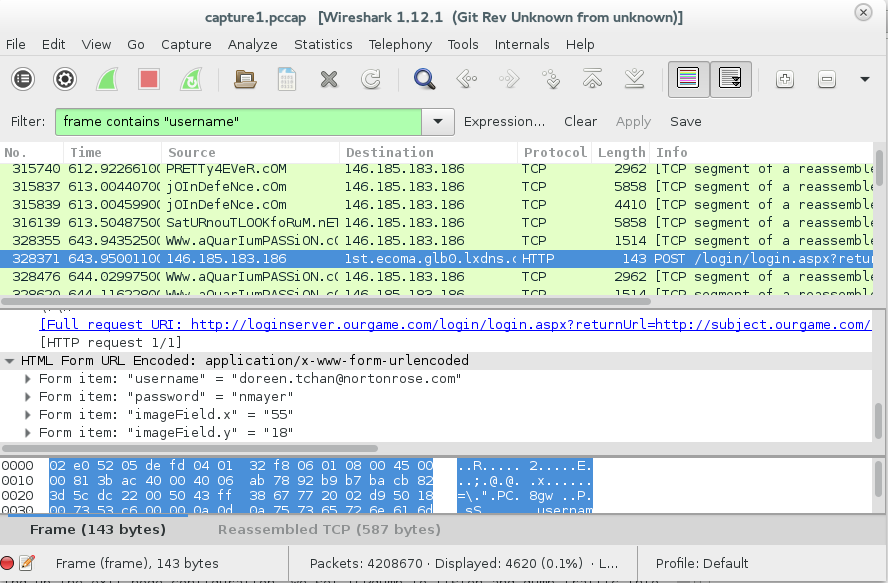
\includegraphics[scale=0.5]{wireshark_username.png}

As is shown in the screenshot above, usernames and passwords sent in cleartext aren't safe even if sent over TOR. Without end-to-end encryption, these are never safe and an exit node can harvest such form data and potentially use these for identifying a target, and access other services used by that target.\\

For TELNET or SMTP packets, we could try to follow the stream for this, and by using tools for deep packet inspection on an exit router it would be possible to inspect packets for email headers containing certain values and store only these, or for packets containing executable files and inject them with a reverse shell or a phone-home call to identify the real location of a target.

These attempts could be thwarted if the target is using Tails or routing his/her traffic through a (physical/virtual) \textit{Whonix} gateway, which forces \textbf{all} traffic through TOR to reduce chances of leaks. 